% AdaScale-CLIP: ICASSP 2027 draft
% Template: spconf.sty (ICASSP/ICIP official style file)
% NOTE: all numeric results come from outputs/ (see scripts/paper/build_tables.py);
%       placeholders marked TODO are filled once EUROSAT/FLO/baseline runs complete.
% --------------------------------------------------------------------------
\pdfminorversion=7
\documentclass{article}
\usepackage{spconf,amsmath,amssymb,graphicx,booktabs,hyperref}
\hypersetup{hidelinks}
\setlength{\dbltextfloatsep}{6pt}\setlength{\textfloatsep}{5pt}\setlength{\floatsep}{5pt}

% Compact author block: drop the blank row after the name row and tighten the
% title area (official fonts/margins unchanged; needed for the 4-page limit).
\makeatletter
\def\name#1{\gdef\@name{{\em #1}}}
\def\@maketitle{\newpage
 \null
 \vskip 1em \begin{center}
 {\large \bf \@title \par} \vskip .75em {\large \lineskip .5em
\begin{tabular}[t]{c}\@name \\ \@address
 \end{tabular}\par} \end{center}
 \par
 \vskip 1em}
\makeatother

\def\x{{\mathbf x}}
\def\w{{\mathbf w}}
\def\f{{\mathbf f}}
\def\p{{\mathbf p}}

\title{AdaScale: Diagnosing and Adapting Multi-Scale Fusion\\ for Training-Free Zero-Shot Recognition}

\name{Dongxu Liu$^{1,\ast}$\thanks{$^{\ast}$Corresponding author.}, Keming Fan$^{2}$, Xiang Luo$^{3}$, Chenrui Zhu$^{3}$, Dongyang Liu$^{4}$}
\address{$^{1}$School of Artificial Intelligence, Jilin University, Changchun, China\\
$^{2}$College of Computer Science and Technology, Jilin University, Changchun, China\\
$^{3}$College of Software, Jilin University, Changchun, China\\
$^{4}$Yingcai Honors College, University of Electronic Science and Technology of China, Chengdu, China\\
{\scriptsize E-mail: liudx9924@mails.jlu.edu.cn, fankm2124@mails.jlu.edu.cn, luoxiang5525@mails.jlu.edu.cn, zhucr5525@mails.jlu.edu.cn, 2024310102018@std.uestc.edu.cn}}

\begin{document}
\sloppy
\maketitle
\vspace{-0.75em}

\begin{abstract}
Zero-shot recognition pipelines built on synthetic class prototypes
combine image crops at multiple scales by fixed
feature fusion. This recipe silently assumes fusion benefits every
target domain. We audit a state-of-the-art pipeline and find two
failure regimes: late scales can overturn correct per-sample
predictions (Oxford-Pets), and, fundamentally, full fusion can be
\emph{systematically worse than the largest single scale across an
entire dataset} (EuroSAT: 42.4\% vs.\ 45.3\%; 36.3\% vs.\ 41.2\%
with synthetic prototypes)---a target-domain property that per-sample
adaptive test-time augmentation cannot diagnose. We propose
\textbf{AdaScale}, a hierarchical training-free controller:
it first compares fused and single-scale prediction entropy on
unlabeled samples to decide whether to fuse for the domain;
within fused domains it stops the scale loop per sample once agreement,
margin, and softmax drift indicate stability, and soft-fuses
evaluated views in probability space. Across Oxford-Pets,
EuroSAT, Flowers-102 and CUB-200 with text and synthetic-image
prototypes (CLIP ViT-B/32), AdaScale matches or exceeds the 10-scale
baseline on all seven settings---improving it by up to
4.8 points---while cutting scale evaluations by up to 90\% and
wall-clock by up to $8.8\times$, and dominates prior-inspired
adaptive-TTA baselines collapsing by up to 8.6 points on the
accuracy--compute Pareto front.
Code is available at \url{https://github.com/ldx825/AdaScale_ICASSP-2027}.
\end{abstract}

\begin{keywords}
zero-shot recognition, vision-language models, test-time augmentation,
adaptive inference, training-free
\end{keywords}

\section{Introduction}
\label{sec:intro}
Contrastive vision-language models such as CLIP~\cite{radford2021clip}
enable zero-shot recognition by matching image features against textual
class prototypes. Recent work shows that \emph{synthetic image}
prototypes---class-conditional images generated by a text-to-image
model---can substantially outperform text prompts as
prototypes~\cite{shi2026lgclip}. The same line of work relies on
multi-scale test-time augmentation: an image is cropped at multiple
scales and the normalized crop features are linearly fused before
matching. The recipe improves robustness to object size and position,
but multiplies inference cost and, as we show, does not help uniformly.

Adaptive test-time augmentation itself is prior art: AdapTTA controls the
number of augmented passes per input, Selective-TTA gates augmentation
by predictive uncertainty, and Intelligent Multi-View TTA decides when
TTA is worthwhile~\cite{mocerino2021adaptta,son2023selective,ozturk2024intelligent};
naive aggregation can flip correct
predictions~\cite{shanmugam2021better}; parameter-updating
TTA~\cite{wang2021tent,sun2020ttt} is orthogonal---AdaScale keeps
the encoder frozen. None of these works addresses the
failure we observe: \emph{the fused predictor can be systematically
inferior to the largest-scale predictor across an entire target domain}.
No per-sample gate we tested can diagnose this: a sample confidently
wrong on small crops passes any confidence-based filter~\cite{guo2017calibration}.

We quantify this with a per-scale utility audit, exposing two failure
regimes. On Oxford-Pets, prefix accuracy (scales $1..s$ fused) peaks at an
intermediate scale and degrades afterwards; 5--10\% of samples are
actively harmed by late scales---motivating sample-wise stopping. On
EuroSAT, more fundamentally, the 10-scale fusion is 3--5 points
\emph{worse} than the largest scale alone in both text and synthetic
prototype pipelines---raising a different question, not \emph{how many}
scales but \emph{whether to fuse at all}. Adaptive multi-scale
inference therefore contains two different decision problems:
\emph{fusion utility is a target-domain property, whereas scale
sufficiency is sample-dependent}.

We propose \textbf{AdaScale}, a hierarchical training-free controller
that separates them. Level~1 diagnoses fusion utility on unlabeled
target samples by comparing the mean prediction entropy of the fused
and single-scale predictors: fusing informative scales ensembles
complementary evidence and reduces uncertainty, whereas fusing
corrupting scales increases it. If the gap exceeds a threshold,
AdaScale runs in \textsc{Single} mode (largest scale only); otherwise
Level~2 stops the scale loop per sample once the running prediction
is stable in margin, consecutive agreement and softmax drift, and a
probability-level soft fusion produces the final output. No labels, no
gradients, and never more scale evaluations than the full baseline.

Our contributions are (i) a \emph{scale-utility audit} identifying two
failure regimes: late scales overturn correct prefix predictions, and
full fusion is systematically worse than the largest scale on an entire
target domain (Sec.~\ref{sec:audit}); (ii) \textbf{AdaScale}, a
hierarchical training-free controller separating a label-free
\emph{fusion-utility diagnosis} from a scale-wise reliability rule with
probability-level soft fusion
(Sec.~\ref{sec:method}); and (iii) experiments on four datasets with
text and synthetic prototypes showing that AdaScale matches or exceeds
the 10-scale baseline on all seven settings (significantly on three, by up
to 4.8 points) at 10--90\% fewer scale evaluations and up to
$8.8\times$ lower wall-clock cost, while prior-inspired adaptive-TTA
baselines collapse by up to 8.6 points (Sec.~\ref{sec:exp}).

\section{Related Work}
\label{sec:related}
\textbf{Synthetic prototypes for zero-shot recognition.}
\cite{shi2026lgclip} uses diffusion-generated class images as prototypes
with multi-scale test-time augmentation; we study the inference-time
utility of its fixed fusion schedule.

\textbf{Adaptive test-time augmentation.}
Prior work shows TTA compute can be allocated adaptively: AdapTTA
controls the number of augmented passes per
input~\cite{mocerino2021adaptta}, Selective-TTA augments only
high-uncertainty samples~\cite{son2023selective}, and Intelligent
Multi-View TTA decides when TTA is
advantageous~\cite{ozturk2024intelligent}; recent work learns an
RL policy in a label-free setting~\cite{mittal2026adaptive}. AdaScale does not claim adaptive
TTA itself as novel. The distinction is the object diagnosed: prior gates
are per-sample, while AdaScale first asks whether the \emph{fusion
operator} helps the target domain---a target-domain property---then
adapts scales per sample.

\textbf{Aggregation and view reliability.}
Shanmugam et al.\ showed that TTA averaging can be suboptimal and can
flip correct predictions~\cite{shanmugam2021better}. Prompt-, adapter-,
and weight-space methods for CLIP adaptation learn or cache
target-specific context~\cite{zhou2022coop,zhou2022cocoop,zhang2022tipadapter,wortsman2022wiseft}.
In CLIP-style test-time adaptation, TPT minimizes entropy over augmented
views with confidence selection~\cite{shu2022tpt} and DiffTPT filters
augmented views by similarity to the test sample~\cite{feng2023difftpt}. These
update prompts or filter views; AdaScale updates no parameters and uses
uncertainty as the diagnostic for whether fusion should be enabled for
the domain.

\textbf{Efficiency in VLMs.}
Encoder/tokenizer efficiency work (learned exit heads,
adaptive-resolution tokenization) is orthogonal~\cite{free2025,lgems2026,lraee2026,waveclip2025,ranet2020,branchynet2016,mobileclip2024}.

\section{Method}
\label{sec:method}

\begin{figure*}[t]
\centering
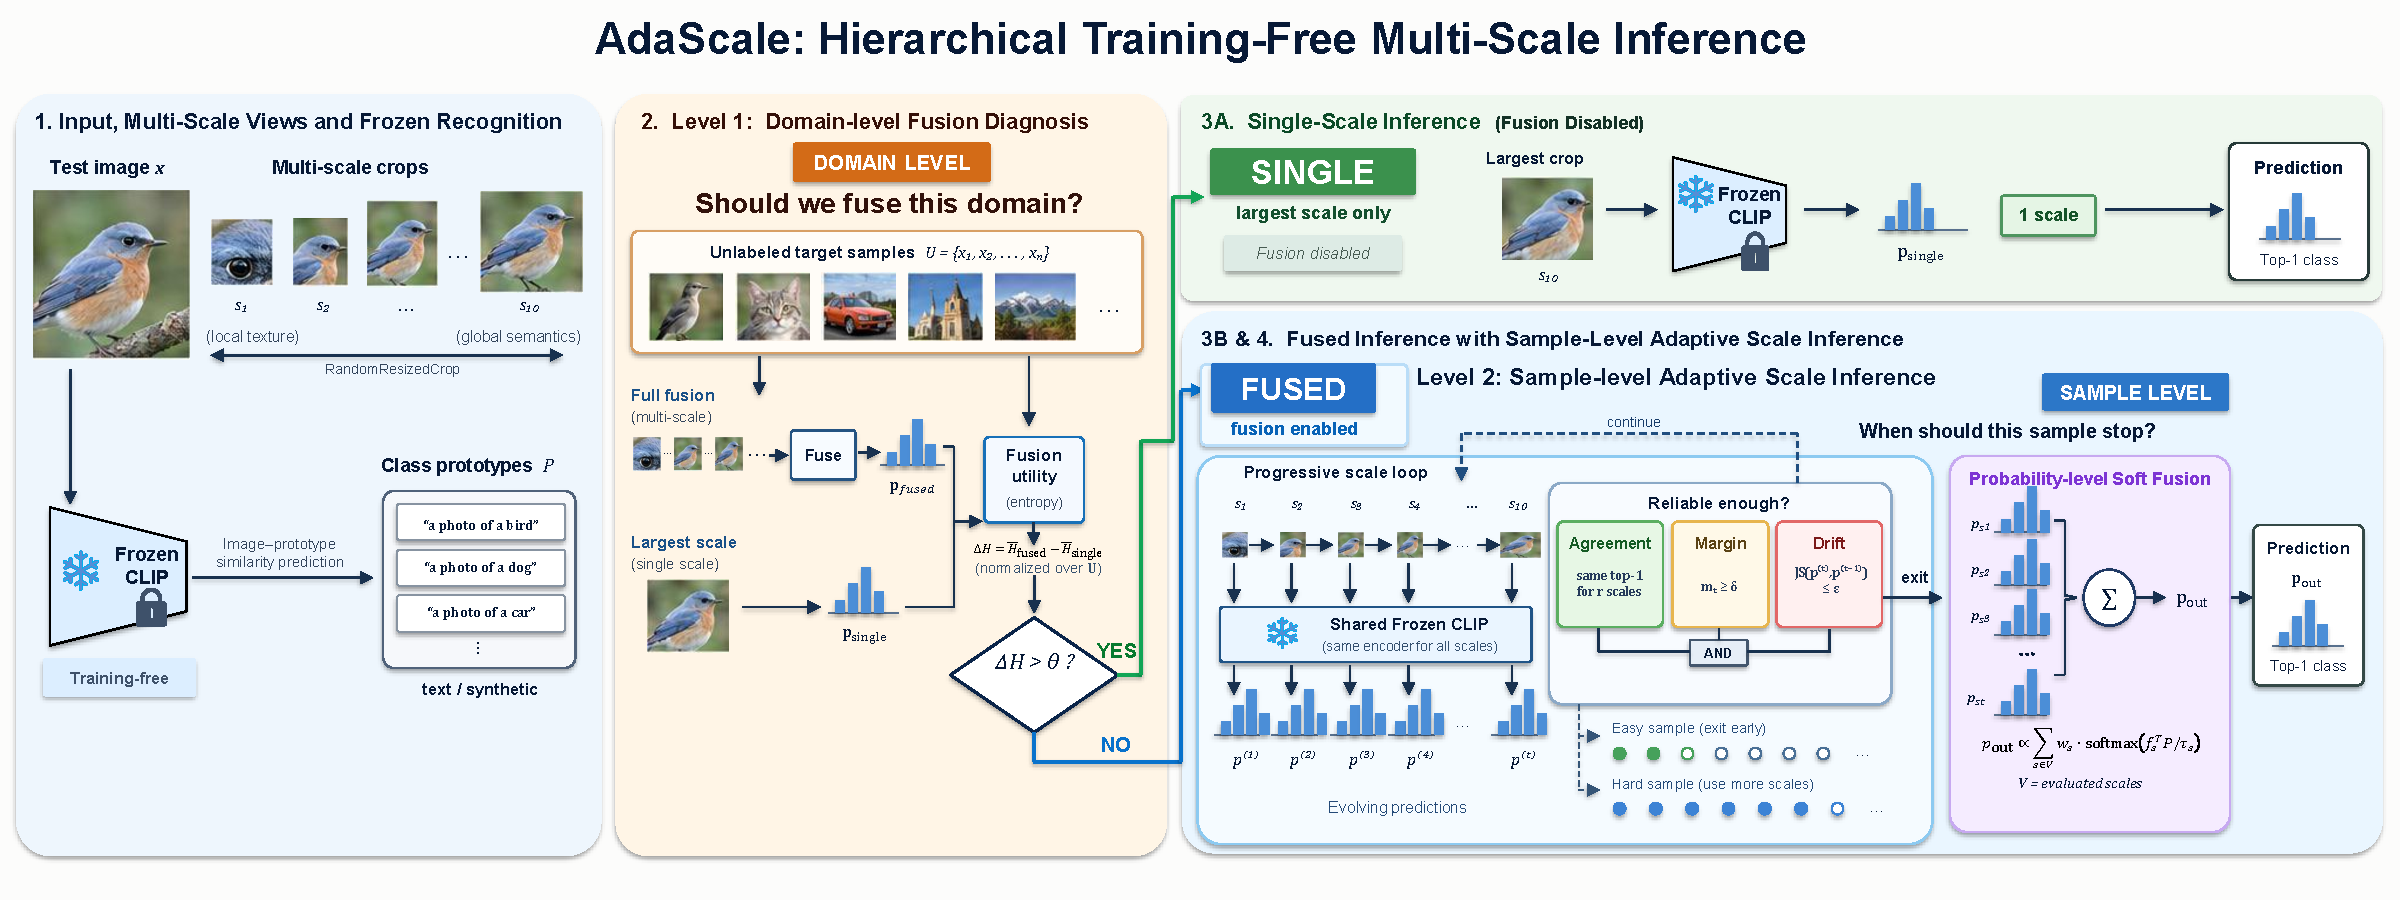
\includegraphics[width=0.88\textwidth]{figures/architecture/AdaScale_high_fidelity_editable.pdf}
\caption{AdaScale: hierarchical training-free multi-scale inference with
a frozen CLIP encoder. Level~1 diagnoses domain-level fusion utility on
unlabeled samples ($\Delta H$ vs.\ $\theta$): \textsc{Single} (3A) uses
the largest scale only; \textsc{Fused} (3B) stops per sample
(agreement/margin/drift) and soft-fuses the evaluated views.}
\label{fig:arch}
\end{figure*}

\subsection{Preliminaries: multi-scale fusion}
Let $x$ be a test image and $\mathcal{S}=\{s_1,\dots,s_S\}$ a set of crop
scales. For each scale $s$, the image is cropped with
$\text{RandomResizedCrop}(224, \text{scale}=(s/10, s/10))$ and encoded
into a normalized feature $f_s \in \mathbb{R}^d$ (frozen CLIP encoder).
Following~\cite{shi2026lgclip}, the
multi-scale feature uses triangular weights $w_s = s / \sum_t t$:
\begin{equation}
\f_{\text{MS}} = \sum_{s \in \mathcal{S}} w_s \, \tilde{f}_s ,
\qquad
\tilde{f}_s = f_s / \|f_s\|_2 ,
\label{eq:fusion}
\end{equation}
and zero-shot logits are
$\ell = \tau^{-1} \f_{\text{MS}}^\top P$, where $P$ collects $C$
prototype features (text or synthetic) and $\tau$ the softmax
temperature ($\tau^{-1}{=}100$ for CLIP).

\subsection{Per-scale utility audit}
\label{sec:audit}
For each sample we compute prefix logits using scales
$\{s_1,\dots,s_t\}$ (weights renormalized over the evaluated subset)
and record cumulative top-1 correctness: (i) the prefix-accuracy
curve, (ii) the fraction of samples \emph{harmed} by later scales
(correct at their best prefix, incorrect at $t{=}S$), (iii) the
minimum equivalent scale $t_{\text{eq}}$, and (iv) the running-margin
ROC-AUC for final stability (Table~\ref{tab:audit}).

\subsection{Unlabeled fusion-utility diagnosis}
\label{sec:mode}
Since fusion is not always beneficial (Sec.~\ref{sec:audit_results}),
AdaScale first decides, without labels, whether to fuse at all---a
\emph{target-domain} decision, not per sample. Given $n$ unlabeled calibration samples:
\begin{equation}
\Delta H = \frac{1}{n}\sum_i
\frac{H\!\left(p^{(S)}_i\right) - H\!\left(p^{(\text{single})}_i\right)}{\log C},
\label{eq:mode}
\end{equation}
where $p^{(S)}$ and $p^{(\text{single})}$ are the fused and largest-scale
predictions. The normalized entropy change is a label-free proxy for
fusion utility: fusing informative scales reduces uncertainty,
corrupting scales increases it. AdaScale runs in
\textsc{Single} mode when $\Delta H > \theta$ ($\theta{=}0.01$)---one
forward pass per image---and in \textsc{Fused} mode otherwise
(sensitivity in the supplementary material).

\subsection{Scale-wise reliability stopping}
\label{sec:adascale}
Building on the general principle of confidence-aware adaptive
TTA~\cite{mocerino2021adaptta,son2023selective}, we instantiate a
scale-wise reliability criterion tailored to prefix multi-scale fusion
(Fig.~\ref{fig:arch}). A sample exits after evaluating scale $s_t$
($t \geq r$) if all three conditions hold:
\begin{align}
\text{(agreement)}\quad & \arg\max p^{(t-j)} \;\text{equal for all } j=0..r{-}1, \\
\text{(margin)}\quad & m_t = p^{(t)}_{(1)} - p^{(t)}_{(2)} \geq \delta, \\
\text{(drift)}\quad & D_{\mathrm{JS}}\!\left(p^{(t)} \,\|\, p^{(t-1)}\right) \leq \varepsilon,
\end{align}
where $p^{(t)}$ is the softmax over the $C$-way logits at temperature
$\tau$. The window guards stale-but-stable tiny crops, the margin
drifting predictions, the drift bound abrupt changes. The rule uses no
labels; one configuration ($r{=}4$, $\delta{=}0.65$, $\varepsilon{=}0.01$)
is frozen for all datasets and prototype types (Sec.~\ref{sec:ablations}).

\subsection{Probability-level soft fusion}
\label{sec:softfusion}
Within \textsc{Fused} mode the output aggregates the evaluated views in
probability space. For the set $\mathcal{V}$ of scales evaluated (a
prefix if it exits early, all scales otherwise):
\begin{equation}
p_{\text{out}} \propto \sum_{s \in \mathcal{V}} w_s \,
\mathrm{softmax}\!\left(\tau_s^{-1} \, f_s^\top P\right),
\label{eq:softfusion}
\end{equation}
with $w_s = s$ and softening temperature $\tau_s = 0.02$. Feature-level
averaging (Eq.~\ref{eq:fusion}) can be dominated by one over-confident
noisy view; softening per-view distributions before averaging makes the
aggregation robust. The temperature is fixed a priori; a single evaluated
view reduces to the standard prediction (\textsc{Single} unchanged).

\section{Experiments}
\label{sec:exp}

\subsection{Setup}
Backbones: CLIP ViT-B/32 (main), ViT-B/16 (validation); prototypes:
text prompts and synthetic images (Stable Diffusion 2.1). Datasets:
Oxford-Pets~\cite{pets2012} (7390 test images), EuroSAT
RGB~\cite{eurosat2019} (27000), Flowers-102~\cite{flowers2008} (8189),
CUB-200-2011~\cite{cub2011} (5794, text only). Runs use one RTX 4080
Super; crops are shared bit-exactly for paired comparison.

\subsection{Scale utility results}
\label{sec:audit_results}
Table~\ref{tab:audit} summarizes the audit; Fig.~\ref{fig:audit} shows
the two regimes side by side. On Oxford-Pets the prefix curve peaks at
an intermediate scale; 5--10\% of samples are harmed by late scales.
On EuroSAT the prefix curve is still monotonic, yet 10-scale fusion
(42.4\%) is 3 points \emph{below} the largest scale alone (45.3\%),
with a larger gap for synthetic prototypes (36.3 vs.\ 41.2\%). The two
datasets represent opposite regimes, indistinguishable without labels.
\begin{figure}[t]
\centering
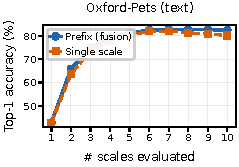
\includegraphics[width=0.47\linewidth]{figures/figA_pet_text.pdf}
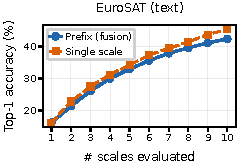
\includegraphics[width=0.47\linewidth]{figures/figA_eurosat_text.pdf}
\caption{Prefix fusion (solid) vs.\ single-scale (dashed). Oxford-Pets
(left): fusion wins. EuroSAT (right): fusion loses to the largest
scale---the schedule must choose per dataset.}
\label{fig:audit}
\end{figure}

\begin{figure*}[!t]
\centering
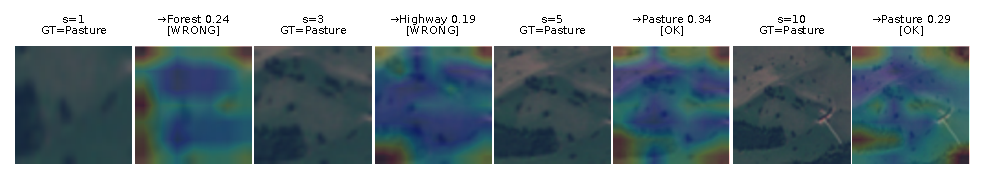
\includegraphics[width=0.97\textwidth]{figures/deep_diag/fig_attn_eurosat.pdf}
\caption{Small-scale damage (EuroSAT/text): at $s{=}1,3$ the crop has
only local texture and the model is wrong; from $s{=}5$ the
global structure is visible and the prediction is correct. Attention
overlays are min--max normalized per crop.}
\label{fig:attn}
\end{figure*}

\begin{table}[t]
\centering
\caption{Scale-utility audit (Pets = Oxford-Pets, Flowers = Flowers-102): prefix-accuracy curve (selected scales), full-10 accuracy, harmful/rescued rate, and median $t_{\mathrm{eq}}$.}
\label{tab:audit}
\small
\setlength{\tabcolsep}{2.5pt}
\begin{tabular}{llcccccr}
\hline
Dataset & Proto & Acc@1 & Acc@5 & Acc@10 & Harm. & Rescue & $t_{eq}$ \\
\hline
Pets & text & 42.9 & 81.2 & 82.4 & 5.0 & 45.4 & 2 \\
Pets & gen & 26.5 & 59.0 & 60.9 & 10.0 & 42.0 & 2 \\
EuroSAT & text & 16.2 & 32.9 & 42.4 & 7.8 & 33.2 & 4 \\
EuroSAT & gen & 11.8 & 22.6 & 36.3 & 2.1 & 25.3 & 1 \\
Flowers & text & 33.3 & 62.9 & 65.1 & 6.0 & 36.1 & 2 \\
Flowers & gen & 21.5 & 41.9 & 42.9 & 9.1 & 27.7 & 3 \\
CUB & text & 16.2 & 51.4 & 53.9 & 10.3 & 43.8 & 3 \\
\hline
\end{tabular}
\end{table}


\subsection{Main results}
\label{sec:main_results}
Table~\ref{tab:main} reports zero-shot accuracy for all seven settings
(probability-level soft fusion adds $+0.14$ points on average across
the five fused-mode settings, all non-negative).
AdaScale matches or exceeds the 10-scale baseline on every setting:
$+2.97$/$+4.84$ (EuroSAT, $p{<}10^{-4}$), $+0.35$ (Flowers-102/gen,
$p{=}0.002$), and $+0.18$/$+0.23$/$+0.05$/$+0.12$ elsewhere
(n.s.; no setting significantly negative). The mode
selector chose \textsc{Single} on both EuroSAT settings and
\textsc{Fused} elsewhere (7/7, 500 unlabeled samples); scale
evaluations drop by 10--90\% (mean 38\%), and fixed-budget truncation
(Fixed-5) loses by 1.4--18.5 points (all $p{<}10^{-3}$). On ViT-B/16, AdaScale attains
86.10\% / 64.49\% on Oxford-Pets (text / synthetic; Full-10:
86.14\% / 64.17\%; $-0.04$ n.s.\ and $+0.32^{*}$) at 36\% / 15\%
savings, reproduces the EuroSAT regime ($+2.27^{*}$), and reaches
68.23\% on Flowers-102/text ($+1.86$).

\begin{table}[t]
\centering
\caption{Zero-shot results (CLIP ViT-B/32; Pets = Oxford-Pets, Flowers = Flowers-102). Full-10: baseline feature fusion. AdaScale auto-selects FUSED (early exit + soft fusion) or SINGLE (largest scale). $\Delta$: paired-bootstrap vs.\ Full-10.}
\label{tab:main}
\small
\setlength{\tabcolsep}{2pt}
\begin{tabular}{llrrcrrr}
\hline
Dataset & Proto & $C$ & Full-10 & Single-10 & AdaScale & $\Delta$ & \#S \\
\hline
Pets & text & 37 & 82.45 & 80.09 & \textbf{82.63} & $+0.18$ & 6.63 \\
Pets & gen & 37 & 60.92 & 57.01 & \textbf{61.15} & $+0.23$ & 8.63 \\
EuroSAT & text & 10 & 42.38 & 45.34 & \textbf{45.34} & $+2.97^{*}$ & 1.00 \\
EuroSAT & gen & 10 & 36.33 & 41.17 & \textbf{41.17} & $+4.84^{*}$ & 1.00 \\
Flowers & text & 102 & 65.12 & 63.05 & \textbf{65.17} & $+0.05$ & 7.91 \\
Flowers & gen & 102 & 42.95 & 41.30 & \textbf{43.30} & $+0.35^{*}$ & 8.92 \\
CUB & text & 200 & 53.90 & 50.22 & \textbf{54.02} & $+0.12$ & 9.01 \\
\hline
\end{tabular}
\end{table}


\subsection{Comparison with prior-inspired adaptive baselines}
\label{sec:baselines}
Table~\ref{tab:baselines} compares AdaScale with adaptive baselines on
identical cached features: \textbf{B1} margin
stopping (AdapTTA-style~\cite{mocerino2021adaptta}: exit at the first
prefix whose margin exceeds a threshold), \textbf{B2} uncertainty
gating (Selective-TTA-style: largest-scale prediction if its entropy is
below threshold, else full fusion), and \textbf{B3} entropy filtering
(5 lowest-entropy views).
Per-sample adaptivity alone is insufficient. B1 collapses on
EuroSAT/gen (27.69\%, $-8.6$): a confidently-wrong prefix passes any
margin threshold, entrenching the failure. B2 never recovers
the single-scale advantage on EuroSAT (44.93/39.46 vs.\ 45.34/41.17 at
exactly $1.0$); on fused domains it needs $9.1$ views on average and
yet only matches the full ten-view baseline, staying below AdaScale's
accuracy at 6.6--8.9 views. B3 needs
\emph{all} ten views (82.75\% on Pets/text) and still cannot fix
EuroSAT (43.42\%). Across both regimes, AdaScale stays on the
accuracy--compute Pareto front; B3 matches it on some settings only by
using all ten views, and trails the single-scale baseline on EuroSAT.
NQ samples (small wrong, large correct) are a third of EuroSAT:
fusion recovers 92--97\% on Pets/Flowers but only 76--85\%
(Fig.~\ref{fig:mech}).

\begin{figure}[t]
\centering
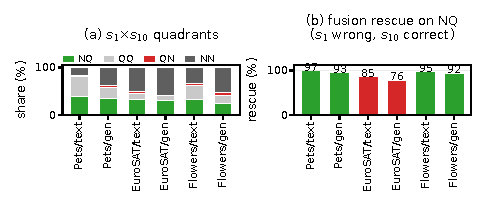
\includegraphics[width=0.98\linewidth]{figures/deep_diag/figM_compact.pdf}
\caption{Microscopic view of the domain-level fusion failure.
(a)~$s_1\times s_{10}$ correctness quadrants ($Q$/N = correct/wrong of
that scale). (b)~Fusion rescue rate on NQ samples (small wrong, large
correct): near-perfect on Pets/Flowers, one fifth lost on EuroSAT.}
\label{fig:mech}
\end{figure}

\begin{table}[t]
\centering
\caption{Comparison with prior-inspired adaptive baselines (accuracy\,\%; subscript: average scale evaluations). B1: margin stopping (AdapTTA-style). B2: uncertainty gating (Selective-TTA-style). B3: keep 5 lowest-entropy views (needs all 10 views). AdaScale: our hierarchical controller.}
\label{tab:baselines}
\scriptsize
\setlength{\tabcolsep}{2.5pt}
\begin{tabular}{llrrrrrr}
\hline
Dataset & Proto & Full-10 & Single-10 & B1 & B2 & B3 & AdaScale \\
\hline
Pets & text & 82.45\,{\tiny 10.0} & 80.09\,{\tiny 1.0} & 82.31\,{\tiny 6.2} & 82.45\,{\tiny 9.1} & 82.75\,{\tiny 10.0} & \textbf{82.63\,{\tiny 6.6}} \\
Pets & gen & 60.92\,{\tiny 10.0} & 57.01\,{\tiny 1.0} & 61.03\,{\tiny 8.9} & 60.92\,{\tiny 9.1} & 61.14\,{\tiny 10.0} & \textbf{61.15\,{\tiny 8.6}} \\
Flowers & text & 65.12\,{\tiny 10.0} & 63.05\,{\tiny 1.0} & 65.08\,{\tiny 8.0} & 65.12\,{\tiny 9.1} & 64.77\,{\tiny 10.0} & \textbf{65.17\,{\tiny 7.9}} \\
Flowers & gen & 42.95\,{\tiny 10.0} & 41.30\,{\tiny 1.0} & 42.94\,{\tiny 9.0} & 42.94\,{\tiny 9.1} & 43.28\,{\tiny 10.0} & \textbf{43.30\,{\tiny 8.9}} \\
EuroSAT & text & 42.38\,{\tiny 10.0} & 45.34\,{\tiny 1.0} & 42.39\,{\tiny 9.8} & 44.93\,{\tiny 1.9} & 43.42\,{\tiny 10.0} & \textbf{45.34\,{\tiny 1.0}} \\
EuroSAT & gen & 36.33\,{\tiny 10.0} & 41.17\,{\tiny 1.0} & 27.69\,{\tiny 5.9} & 39.46\,{\tiny 1.9} & 36.00\,{\tiny 10.0} & \textbf{41.17\,{\tiny 1.0}} \\
CUB & text & 53.90\,{\tiny 10.0} & 50.22\,{\tiny 1.0} & 53.88\,{\tiny 9.1} & 53.90\,{\tiny 9.1} & 54.25\,{\tiny 10.0} & \textbf{54.02\,{\tiny 9.0}} \\
\hline
\end{tabular}
\end{table}


\enlargethispage{4\baselineskip}
\subsection{Ablations}
\label{sec:ablations}
{\small
\textbf{Stability configuration.}
$r{=}4,\delta{=}0.65,\varepsilon{=}0.01$ attains the best worst-case
delta among searched configurations ($-0.07$, n.s.);
$\delta{=}0.45$ trades $0.07$--$0.20$ accuracy for six points of
compute savings; calibration robustness is in the supplement.
}

\subsection{Runtime analysis}
\label{sec:runtime}
Wall-clock timing (RTX 4080 Super): AdaScale is 1.44$\times$ faster
than Full-10 on Oxford-Pets; EuroSAT single-scale execution is
$8.8\times$ faster ($45$s vs.\ $397$s for 27k images) at higher
accuracy---redundant scales are wasteful and harmful. Method timings are
in the supplement.

% Table 4 (runtime) moved to supplementary material: paper/tables/tab_runtime.tex
% \begin{table}[t]
\centering
\caption{Wall-clock inference (batch 32, RTX 4080 Super). PET: $N{=}7390$; EuroSAT: $N{=}27000$; Single mode evaluates only the largest scale.}
\label{tab:runtime}
\small
\setlength{\tabcolsep}{4pt}
\begin{tabular}{lrrrr}
\hline
Method & Time (s) & Ips. & Acc (\%) & Avg. scales \\
\hline
Full-10 (PET) & 290 & 25.4 & 82.50 & 10.00 \\
Fixed-5 (PET) & 127 & 58.3 & 81.15 & 5.00 \\
Fixed-7 (PET) & 189 & 39.0 & 82.75 & 7.00 \\
AdaScale (PET) & 202 & 36.6 & 82.37 & 6.64 \\
Full-10 (EURO; 27k) & 397 & 68.0 & 42.35 & 10.00 \\
Single (EURO; 27k) & 45 & 595.8 & 45.34 & 1.00 \\
\hline
\end{tabular}
\end{table}


\enlargethispage{3.5\baselineskip}
\section{Conclusion}
Fixed multi-scale fusion assumes fusion helps every domain---but on
EuroSAT, fusing all scales is systematically worse than the largest
single scale (42.4\% vs.\ 45.3\%), a target-domain failure that
per-sample gates cannot diagnose. We address it with AdaScale: a
training-free controller that first decides whether a domain should
fuse at all, then stops each sample once its fused prediction
stabilizes. Across four datasets with text and synthetic prototypes,
it matches or exceeds the 10-scale baseline---by up to 4.8
points---while evaluating up to 90\% fewer scales.

\clearpage
\ninept
\bibliographystyle{IEEEbib}
\bibliography{adascale}

\end{document}
